\documentclass[../main]{subfiles}

\questiontrue
\solutiontrue

\begin{document}
    \ifquestion
    
	
\section{Non-Homogeneous Cosmology}

\parte{A}{Spherical Cavity}

One of the universes in the multiverse is non-homogeneous. It is a sphere of matter density equal to $\rho$ that has a spherical cavity at a distance $a$ from the center. Inside this cavity, there is a total absence of matter, as shown in \autoref{fig:nonhomogeneus}.


	\begin{figure}[htpb]
	    \centering
	    

\tikzset{every picture/.style={line width=0.75pt}} %set default line width to 0.75pt        

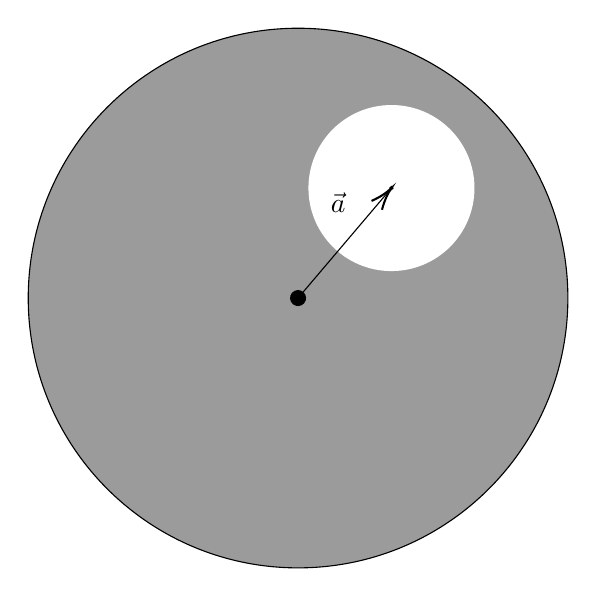
\begin{tikzpicture}[x=0.75pt,y=0.75pt,yscale=-1,xscale=1]
%uncomment if require: \path (0,408); %set diagram left start at 0, and has height of 408

%Shape: Circle [id:dp869407249172657] 
\draw  [fill={rgb, 255:red, 155; green, 155; blue, 155 }  ,fill opacity=1 ] (174,183) .. controls (174,111.2) and (232.2,53) .. (304,53) .. controls (375.8,53) and (434,111.2) .. (434,183) .. controls (434,254.8) and (375.8,313) .. (304,313) .. controls (232.2,313) and (174,254.8) .. (174,183) -- cycle ;
%Shape: Circle [id:dp2950696170902345] 
\draw  [color={rgb, 255:red, 0; green, 0; blue, 0 }  ,draw opacity=0 ][fill={rgb, 255:red, 255; green, 255; blue, 255 }  ,fill opacity=1 ] (309,130) .. controls (309,107.91) and (326.91,90) .. (349,90) .. controls (371.09,90) and (389,107.91) .. (389,130) .. controls (389,152.09) and (371.09,170) .. (349,170) .. controls (326.91,170) and (309,152.09) .. (309,130) -- cycle ;
%Straight Lines [id:da6146869915357251] 
\draw    (347.71,131.52) -- (304,183) ;
\draw [shift={(304,183)}, rotate = 130.33] [color={rgb, 255:red, 0; green, 0; blue, 0 }  ][fill={rgb, 255:red, 0; green, 0; blue, 0 }  ][line width=0.75]      (0, 0) circle [x radius= 3.35, y radius= 3.35]   ;
\draw [shift={(349,130)}, rotate = 130.33] [color={rgb, 255:red, 0; green, 0; blue, 0 }  ][line width=0.75]    (10.93,-3.29) .. controls (6.95,-1.4) and (3.31,-0.3) .. (0,0) .. controls (3.31,0.3) and (6.95,1.4) .. (10.93,3.29)   ;
%Shape: Circle [id:dp2190094298644336] 
\draw  [fill={rgb, 255:red, 0; green, 0; blue, 0 }  ,fill opacity=1 ] (348.25,130) .. controls (348.25,129.59) and (348.59,129.25) .. (349,129.25) .. controls (349.41,129.25) and (349.75,129.59) .. (349.75,130) .. controls (349.75,130.41) and (349.41,130.75) .. (349,130.75) .. controls (348.59,130.75) and (348.25,130.41) .. (348.25,130) -- cycle ;

% Text Node
\draw (318.5,131.07) node [anchor=north west][inner sep=0.75pt]    {$\vec{a}$};


\end{tikzpicture}
	
\caption{Composition and distribution of matter in the universe under consideration}
\label{fig:nonhomogeneus}
\end{figure}

\ut{A.1} Find a relation for the gravitational field inside the cavity.

Hint: Think about the superposition of matter and remember the vectorial analysis of gravitation.

\parte{B}{Discrete Distribution}

A similar situation occurs in universe M190i, a non-homogeneous universe consisting of an inner sphere with energy density $\epsilon_b$ and a spherical shell with energy density $\epsilon_a$, as shown in the figure:

	\begin{figure}[htpb]
	    \centering
	    

\tikzset{every picture/.style={line width=0.75pt}} %set default line width to 0.75pt        

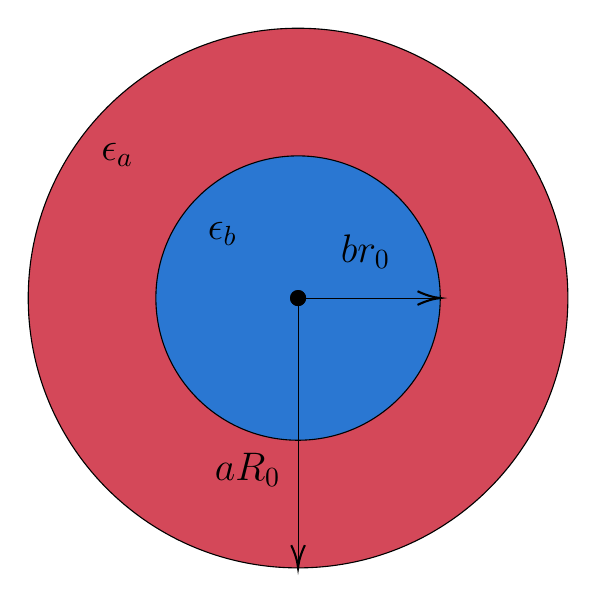
\begin{tikzpicture}[x=0.75pt,y=0.75pt,yscale=-1,xscale=1]
%uncomment if require: \path (0,408); %set diagram left start at 0, and has height of 408

%Shape: Circle [id:dp869407249172657] 
\draw  [fill={rgb, 255:red, 212; green, 72; blue, 89 }  ,fill opacity=1 ] (174,183) .. controls (174,111.2) and (232.2,53) .. (304,53) .. controls (375.8,53) and (434,111.2) .. (434,183) .. controls (434,254.8) and (375.8,313) .. (304,313) .. controls (232.2,313) and (174,254.8) .. (174,183) -- cycle ;
%Shape: Circle [id:dp2950696170902345] 
\draw  [color={rgb, 255:red, 0; green, 0; blue, 0 }  ,draw opacity=1 ][fill={rgb, 255:red, 42; green, 119; blue, 210 }  ,fill opacity=1 ] (235.5,183) .. controls (235.5,145.17) and (266.17,114.5) .. (304,114.5) .. controls (341.83,114.5) and (372.5,145.17) .. (372.5,183) .. controls (372.5,220.83) and (341.83,251.5) .. (304,251.5) .. controls (266.17,251.5) and (235.5,220.83) .. (235.5,183) -- cycle ;
%Straight Lines [id:da6146869915357251] 
\draw    (370.5,183) -- (304,183) ;
\draw [shift={(304,183)}, rotate = 180] [color={rgb, 255:red, 0; green, 0; blue, 0 }  ][fill={rgb, 255:red, 0; green, 0; blue, 0 }  ][line width=0.75]      (0, 0) circle [x radius= 3.35, y radius= 3.35]   ;
\draw [shift={(372.5,183)}, rotate = 180] [color={rgb, 255:red, 0; green, 0; blue, 0 }  ][line width=0.75]    (10.93,-3.29) .. controls (6.95,-1.4) and (3.31,-0.3) .. (0,0) .. controls (3.31,0.3) and (6.95,1.4) .. (10.93,3.29)   ;
%Straight Lines [id:da5288386645098062] 
\draw    (304,311) -- (304,183) ;
\draw [shift={(304,183)}, rotate = 270] [color={rgb, 255:red, 0; green, 0; blue, 0 }  ][fill={rgb, 255:red, 0; green, 0; blue, 0 }  ][line width=0.75]      (0, 0) circle [x radius= 3.35, y radius= 3.35]   ;
\draw [shift={(304,313)}, rotate = 270] [color={rgb, 255:red, 0; green, 0; blue, 0 }  ][line width=0.75]    (10.93,-3.29) .. controls (6.95,-1.4) and (3.31,-0.3) .. (0,0) .. controls (3.31,0.3) and (6.95,1.4) .. (10.93,3.29)   ;

% Text Node
\draw (323.33,151.41) node [anchor=north west][inner sep=0.75pt]  [font=\Large]  {$br_{0}$};
% Text Node
\draw (262.67,256.74) node [anchor=north west][inner sep=0.75pt]  [font=\Large]  {$aR_{0}$};
% Text Node
\draw (259.33,145.08) node [anchor=north west][inner sep=0.75pt]  [font=\Large]  {$\epsilon _{b}$};
% Text Node
\draw (208,107.08) node [anchor=north west][inner sep=0.75pt]  [font=\Large]  {$\epsilon _{a}$};


\end{tikzpicture}
	
\caption{Density map of the M190i universe}
\label{fig:M190i}
\end{figure}

Let $b$ and $a$ be the scale factors for the inner and outer parts, respectively, and $r_0$ and $R_0$ the initial radii of the inner and outer parts, respectively.

In this problem, use $H_x = \dfrac{\dot{x}}{x}$ and $\Omega_x = \dfrac{\epsilon_x}{\epsilon_{x,c}}$, where $\epsilon_{x,c}$ is the critical energy density of parameter $x$. Also, take that parameters with subscript 0 refer to current values.

\ut{B.1} Show that the evolution relation of the inner part is given by:

\[
H_b^2=\frac{8\pi G}{3c^2}\epsilon_b
\]

\ut{B.2} Now analyze the evolution law of the shell. Show that:

\[
H_a^2=\frac{8\pi G}{3c^2}\epsilon_a\left(1+\left(\frac{br_0}{aR_0}\right)^3\left(\frac{\epsilon_b}{\epsilon_a}-1\right)\right)
\]

A cosmologist from this universe noticed that, coincidentally, the gravitational field inside the inner region (with energy density $\epsilon_b$) was constant.

\ut{B.3} An interesting factor about the relation for energy density as a function of the scale factor comes from dark energy: it has been observed that such dependence is $\dfrac{d\epsilon_a}{dt}=0$, so find the evolution function of the universe's shell.

Hint: When the integral becomes painful, a substitution like $u=\sqrt{1-za^{-m}}$ might help a lot. Also use:

\[
\int \frac{dx}{1-x^2} = \tanh^{-1}{x} + C
\]

\clearpage

\fi

\ifsolution

\section{Non-Homogeneous Cosmology}

\parte{A}{Spherical Cavity}

\ut{A.1} Imagine that the cavity inside the sphere is the superposition of a sphere of mass $m$ with another sphere of mass $-m$ (because in the end they cancel each other out). Thus, we can calculate the field at a point in space as the sum of the field generated by the full sphere and by a sphere of the same density magnitude but negative.

For a person inside a sphere, the field at a point is only due to the sphere inside them. So, the field generated by the larger sphere at a point with position vector $\vec{r}$ relative to the sphere's center is:

\[
\vec{g}_1=-\frac{GM_i}{r^2}\hat{r}
\]

where $M_i=\dfrac{4}{3}\pi r^3 \rho$ (internal mass), hence:

\[
\vec{g}_1=-4\pi G \rho \vec{r}
\]

For the sphere of density $\rho$, we have $\vec{r}_2=\vec{r}-\vec{a}$ (relative position to the center). Analogously:

\[
\vec{g}_2=4\pi G \rho \vec{r}_2=4\pi G \rho \vec{r} - 4\pi G \rho \vec{a}
\]

Adding the two fields vectorially, we get:

\[
\vec{g}_t= -4\pi G \rho \vec{a}
\]

Notice that the field is constant and points in a constant direction.

\parte{B}{Discrete Distribution}

\ut{B.1} For the inner part, we can simply use the classical demonstration of the Friedmann law since the shell does not influence the development of the inner part (easily seen via Gauss's law for gravitation, also known as the shell theorem):

Consider a reference point at a distance $br_0$ from the universe's center, using the gravitational Gauss law:

\[
\oint\vec{g}\cdot\vec{dA}=-4\pi G m_i
\]

Since $|\vec{g}|$ is constant and always perpendicular to the area elements:

\[
\vec{g}\oint\cdot\vec{dA}=\vec{g}4\pi r^2=-4\pi G m_i
\]

\[
\vec{g}=-\frac{Gm_i}{r^2}\hat{r}
\]

Considering mass conservation in the expansion and $g=\dfrac{d^2r}{dt^2}=\dfrac{dv}{dt}$, integrate the expression in terms of $dr$:

\[
\int \frac{dv}{dt}dx=-Gm_i\int r^{-2}dr
\]

\[
\int v dv =\frac{Gm_i}{r}+C
\]

\[
v^2 =\frac{2Gm_i}{r}+C'
\]

Now note that $m_i=\frac{4}{3}\pi r^3 \rho$, and we can write $r$ and $v$ as $br_0$ and $\dot{b}r_0$, respectively.

\[
\dot{b}^2=\frac{8\pi G}{3}\rho b^2 + C''
\]

Dividing both sides by $b^2$ and noting that $C''=0$ for a flat universe:

\[
\left(\frac{\dot{b}}{b}\right)^2=\frac{8 \pi G}{3} \rho
\]

Since $H_b = \dfrac{\dot{b}}{b}$ and relativistic energy includes the factor $c^2$ from $E=mc^2$:

\[
H_b^2=\frac{8 \pi G}{3c^2}\epsilon_{b}
\]

\ut{B.2} For the outer sphere, we can follow the same procedure, but now the internal mass is dictated by another relation. Still:

\[
v^2 =\frac{2Gm_i}{r}+C''
\]

Here we consider the superposition of a larger sphere with density $\rho_a$ and a smaller sphere with density $\rho_b-\rho_a$, so that the total density in the intersection region (smaller sphere) is $\rho_b$.

Now $r=aR_0$, $v=R_0\dot{a}$, and 

\[
m_i = \dfrac{4 \pi b^3r_0^3}{3}(\rho_b-\rho_a)+\dfrac{4 \pi a^3 R_0^3}{3}\rho_a
\]

Rewriting:

\[
\dot{a}^2R_0^2=\frac{8\pi G}{3aR_0}\left(b^3r_0^3(\rho_b-\rho_a)+a^3R_0^3\rho_a\right)
\]

Simplifying:

\[
\dot{a}^2=\frac{8\pi G}{3}\left(\left(\frac{br_0}{aR_0}\right)^3\frac{\epsilon_b-\epsilon_a}{c^2}+\frac{\epsilon_a}{c^2}\right)
\]

Finally:

\[
H_a^2=\frac{8\pi G}{3c^2}\epsilon_a\left(1+\left(\frac{br_0}{aR_0}\right)^3\left(\frac{\epsilon_b}{\epsilon_a}-1\right)\right)
\]

\ut{B.3} For the gravitational field inside the inner region to be constant, it is necessary that $\epsilon_b=0$ (any other value would create a central attractive force). Substituting $\epsilon_b=0$:

\[
H_b^2=0 \therefore \dot{b}=0
\]

So $b$ is constant: $b=b_0=1$. Then:

\[
H_a^2=\frac{8\pi G}{3c^2}\epsilon_a\left(1-1\left(\frac{r_0}{aR_0}\right)^3\right)
\]

Isolating $\dot{a}$:

\[
\dot{a}^2=\frac{8 \pi G}{3c^2}\epsilon_aa^2\left(1-1\left(\frac{r_0}{aR_0}\right)^3\right)
\]

Assuming $\epsilon_a$ is constant over time:

\[
\dot{a}^2=\frac{8 \pi G}{3c^2}\epsilon_{a,0}a^{2}\left(1-1\left(\frac{r_0}{aR_0}\right)^3\right)
\]

Let $n=\dfrac{8 \pi G}{3c^2}\epsilon_{a,0}$ and $m=\dfrac{r_0^3}{R_0^3}$:

\[
\dot{a}^2=na^{2}\left(1-ma^{-3}\right)
\]

\[
\dot{a}=\sqrt{n}a\sqrt{1-ma^{-3}}
\]

Separating variables to integrate:

\[
\int_1^a a^{-1}\frac{da}{\sqrt{1-ma^{-3}}}=\int_{t_0}^t \sqrt{n}dt
\]

Using the suggested substitution $u=\sqrt{1-ma^{-3}}$:

\[
du=\frac{3ma^{-4}da}{2\sqrt{1-ma^{-3}}}
\]

Substituting:

\[
\frac{2a^4du}{3m}=\frac{da}{\sqrt{1-ma^{-3}}}
\]

\[
\int_{\sqrt{1-m}}^{\sqrt{1-ma^{-3}}} a^{3}\frac{2du}{3m}=\int_{t_0}^t \sqrt{n}dt
\]

Since $a=\left(\frac{1-u^2}{m}\right)^{-\frac{1}{3}}$, the integral becomes:

\[
\int_{\sqrt{1-m}}^{\sqrt{1-ma^{-3}}} \frac{m}{1-u^2}\frac{2du}{3m}=\int_{t_0}^t \sqrt{n}dt
\]

Simplifying:

\[
\int_{\sqrt{1-m}}^{\sqrt{1-ma^{-3}}} \frac{du}{1-u^2}=\frac{3}{2}\Delta t \sqrt{n}
\]

Knowing that:

\[
\int \frac{du}{1-u^2} = \tanh^{-1}{u} + C
\]

Thus we find:

\[
\tanh^{-1}{\sqrt{1-ma^{-3}}}-\tanh^{-1}{\sqrt{1-m}}=\frac{3}{2}\Delta t \sqrt{n}
\]

Assuming $t_0=0$ (present):

	$$a(t)=\left(\frac{m}{1-\tanh^2{\left(\tanh^{-1}{\sqrt{1-m}}+\frac{3}{2}t \sqrt{n}\right)}}\right)^{\frac{1}{3}}$$
	
	$$a(t)=\frac{r_0}{R_0}\left(1-\tanh^2{\left(\tanh^{-1}{\sqrt{1-\frac{r_0^3}{R_0^3}}}+\frac{3}{2}t \sqrt{\frac{8 \pi G}{3c^2}\epsilon_{a,0}}\right)}\right)^{-\frac{1}{3}}$$

    
 
	\clearpage
    
    
    \fi
\end{document}
